% Created 2020-03-26 jue 09:43
% Intended LaTeX compiler: pdflatex
\documentclass[presentation,aspectratio=169]{beamer}
\usepackage[utf8]{inputenc}
\usepackage[T1]{fontenc}
\usepackage{graphicx}
\usepackage{grffile}
\usepackage{longtable}
\usepackage{wrapfig}
\usepackage{rotating}
\usepackage[normalem]{ulem}
\usepackage{amsmath}
\usepackage{textcomp}
\usepackage{amssymb}
\usepackage{capt-of}
\usepackage{hyperref}
\usepackage{khpreamble}
\usetheme{default}
\author{Kjartan Halvorsen}
\date{\today}
\title{Process automation laboratory - Root locus, PI control}
\hypersetup{
 pdfauthor={Kjartan Halvorsen},
 pdftitle={Process automation laboratory - Root locus, PI control},
 pdfkeywords={},
 pdfsubject={},
 pdfcreator={Emacs 26.3 (Org mode 9.3.6)}, 
 pdflang={English}}
\begin{document}

\maketitle

\section{Intro}
\label{sec:org71aeb1b}

\begin{frame}[label={sec:orga305772}]{Repetition: The RC-circuit - a first-order system}
\begin{center}
\begin{tikzpicture}
\node (circuit) {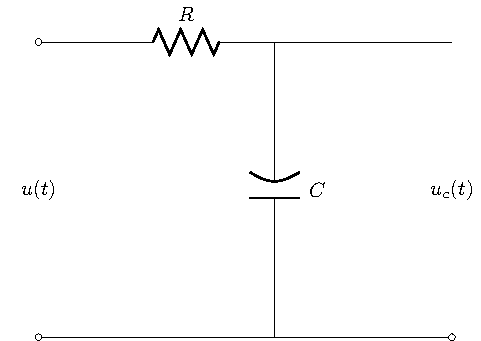
\includegraphics[width=0.4\linewidth]{../../figures/RC-input-output.pdf}};
\begin{scope}[xshift=6cm, yshift=-0.8cm]
  \draw[->] (-2,0) to (1,0);
  \draw[->] (0,-1) to (0,1);
  \node at (1,1) {$s$-plane};
  \node[color=red!80!black] (pole) at (-1.2, 0) {\large $\times$};
  \node[below of=pole, node distance=5mm, ] {$-\frac{1}{\tau}$};
\end{scope}
\node (laplace) at(6,1.5)  {$U_C(s) = \frac{1}{s\underbrace{RC}_{\tau} + 1} U(s)$};
\begin{axis}[
yshift=-5cm,
clip=false,
width = 12cm,
height = 3.5cm,
xlabel = {$t$},
ylabel = {V},
title = {$u_C(t) = 10 (1 - \mathrm{e}^{\frac{t}{\tau}})$, for $u(t)$ step of size 10},
]
\addplot[blue!80!black, thick, no marks, const plot] coordinates {
(-0.2,0)
(0,10)
(2,0)
(4,10)
(6,0)
} node[coordinate, pos=0.75, pin=180:{$u(t)$}] {};
\addplot[orange!80!black, thick, no marks, domain=-0.2:0, samples=2] {0};
\addplot[orange!90!black, thick, no marks, domain=0:2, samples=40] {10*(1-exp(-x/0.2)};
\addplot[orange!90!black, thick, no marks, domain=4:6, samples=40] {10*(1-exp(-(x-4)/0.2)} node[coordinate, pos=0.84, pin=-90:{$u_C(t)$}] {};
\addplot[orange!90!black, thick, no marks, domain=2:4, samples=40] {10*exp(-(x-2)/0.2)};
\end{axis}

\end{tikzpicture}
\end{center}
\end{frame}
\begin{frame}[label={sec:org6050dc7}]{A concept to keep in mind}
In a system with an \alert{integrator} steady-state can only exist if the signal to the integrator is zero

\begin{center}
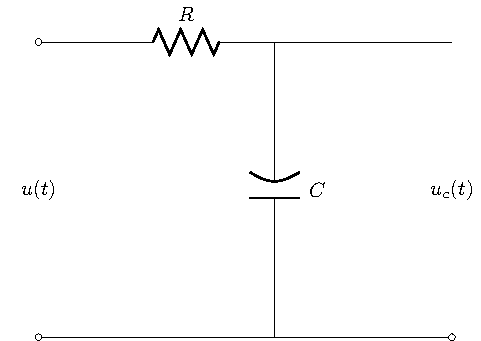
\includegraphics[width=0.4\linewidth]{../../figures/RC-input-output.pdf}
\end{center}

\begin{center}
  \begin{tikzpicture}[scale = 0.8, node distance=25mm, block/.style={rectangle, draw, minimum width=15mm}, sumnode/.style={circle, draw, inner sep=2pt}]

  \node[coordinate] (input) {};
  \node[block, right of=input] (cap) {$C$};
  \node[coordinate, right of=cap] (output) {};

  \draw[->] (finput) -- node[above, pos=0.3] {$i(t)$} (cap);
  \draw[->] (cap) -- node[above, pos=0.7] {$u_C(t)$} (output);

  \node[right of=output, node distance=40mm] {$u_C(t) = u_C(0) + \frac{1}{C}\int i(s) ds$};
  \end{tikzpicture}
\end{center}
\end{frame}



\begin{frame}[label={sec:org7077543}]{Feedback control}
\begin{center}
  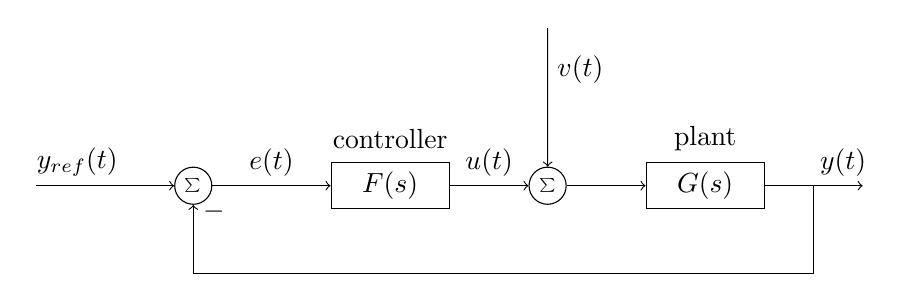
\begin{tikzpicture}[scale = 0.8, node distance=25mm, block/.style={rectangle, draw, minimum width=15mm}, sumnode/.style={circle, draw, inner sep=2pt}]

  \node[coordinate] (refinput) {};
  \node[sumnode, right of=refinput, node distance=20mm] (sumerr) {\tiny $\sum$};
  \node[block, right of=sumerr] (controller) {$F(s)$};
  \node[above of=controller, node distance=6mm] {controller};
  \node[sumnode, right of=controller, node distance=20mm] (sumdist) {\tiny $\sum$};
  \node[block, right of=sumdist, node distance=20mm] (plant) {$G(s)$};
  \node[above of=plant, node distance=6mm] {plant};
  \node[coordinate, right of=plant, node distance=20mm] (output) {};
  \node[coordinate, above of=sumdist, node distance=20mm] (dist) {};

  \draw[->] (refinput) -- node[above, pos=0.3] {$y_{ref}(t)$} (sumerr);
  \draw[->] (sumerr) -- node[above] {$e(t)$} (controller);
  \draw[->] (controller) -- node[above] {$u(t)$} (sumdist);
  \draw[->] (sumdist) -- node[above] {$$} (plant);
  \draw[->] (plant) -- node[coordinate] (measure) {} node[above, pos=0.8] {$y(t)$} (output);
  \draw[->] (measure) -- ++(0,-14mm) -| node[right, pos=0.95] {$-$} (sumerr);
  \draw[->] (dist) -- node[right, pos=0.3] {$v(t)$} (sumdist);

  \end{tikzpicture}
\end{center}

For the closed-loop system we get
\[ Y(s) = \frac{G_o(s)}{1+G_o(s)}Y_{ref}(s) + \frac{G(s)}{1 + G_o(s)} V(s), \]
where \(G_o(s)=G(s)F(s)\) is called the \emph{loop gain}.
\end{frame}

\begin{frame}[label={sec:orgc4b7770}]{Feedback control}
\begin{center}
  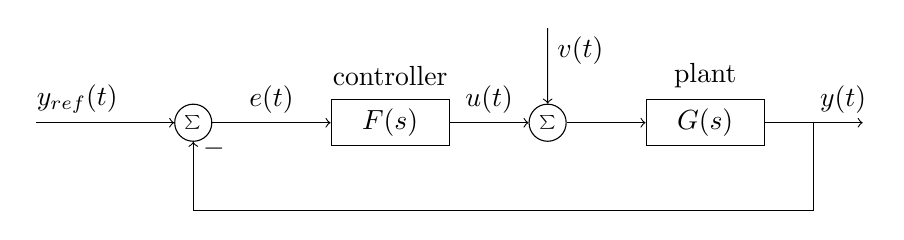
\begin{tikzpicture}[scale = 0.8, node distance=25mm, block/.style={rectangle, draw, minimum width=15mm}, sumnode/.style={circle, draw, inner sep=2pt}]

  \node[coordinate] (refinput) {};
  \node[sumnode, right of=refinput, node distance=20mm] (sumerr) {\tiny $\sum$};
  \node[block, right of=sumerr] (controller) {$F(s)$};
  \node[above of=controller, node distance=6mm] {controller};
  \node[sumnode, right of=controller, node distance=20mm] (sumdist) {\tiny $\sum$};
  \node[block, right of=sumdist, node distance=20mm] (plant) {$G(s)$};
  \node[above of=plant, node distance=6mm] {plant};
  \node[coordinate, right of=plant, node distance=20mm] (output) {};
  \node[coordinate, above of=sumdist, node distance=12mm] (dist) {};

  \draw[->] (refinput) -- node[above, pos=0.3] {$y_{ref}(t)$} (sumerr);
  \draw[->] (sumerr) -- node[above] {$e(t)$} (controller);
  \draw[->] (controller) -- node[above] {$u(t)$} (sumdist);
  \draw[->] (sumdist) -- node[above] {$$} (plant);
  \draw[->] (plant) -- node[coordinate] (measure) {} node[above, pos=0.8] {$y(t)$} (output);
  \draw[->] (measure) -- ++(0,-14mm) -| node[right, pos=0.95] {$-$} (sumerr);
  \draw[->] (dist) -- node[right, pos=0.3] {$v(t)$} (sumdist);

  \end{tikzpicture}
\end{center}

\[ Y(s) = \frac{G_o(s)}{1+G_o(s)}Y_{ref}(s) + \frac{G(s)}{1+G_o(s)}V(s), \quad G_o(s)=G(s)F(s). \]

Let \(G(s) = \frac{1}{s}\) and \(F(s)=K\). 
\begin{enumerate}
\item Will there be a steady-state control error (\(\lim_{t\to\infty} e(t)\)  \(\neq\) 0) if \(y_{ref}(t)=0\) and \(v(t)\) is a unit step? Why? \alert{Answer on Socrative}
\item What is the \alert{characteristic equation} for the closed-loop system?
\item Sketch the location of the poles in the imaginary plane as the gain \(K\) varies from 0 to \(\infty\). \alert{Group exercise in breakout room}
\end{enumerate}
\end{frame}


\begin{frame}[label={sec:orgad4a3db}]{How to get rid of the steady-state error}
Use a proportional-integral controller (PI controller)
\[ F(s) = K_p + \frac{K_i}{s}. \]
This gives closed-loop system

\begin{center}
   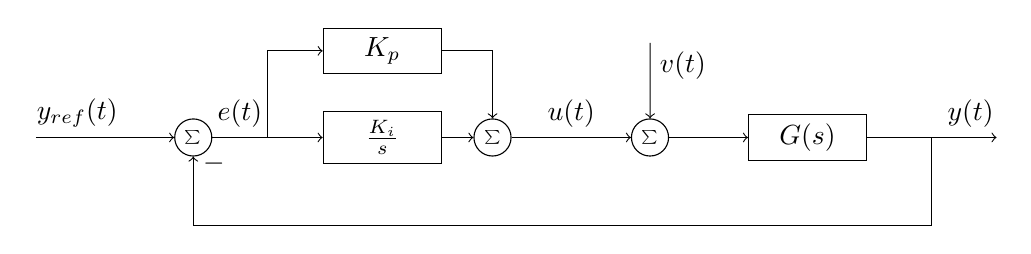
\begin{tikzpicture}[scale = 0.8, node distance=20mm, block/.style={rectangle, draw, minimum width=15mm}, sumnode/.style={circle, draw, inner sep=2pt}]

   \node[coordinate] (refinput) {};
   \node[sumnode, right of=refinput, node distance=20mm] (sumerr) {\tiny $\sum$};
   \node[block, right of=sumerr, node distance=24mm] (Ipart) {$\frac{K_i}{s}$};
   \node[block, above of=Ipart, node distance=11mm] (Ppart) {$K_p$};
   \node[sumnode, right of=Ipart, node distance=14mm] (sumcontrol) {\tiny $\sum$};
   \node[sumnode, right of=sumcontrol, node distance=20mm] (sumdist) {\tiny $\sum$};
   \node[block, right of=sumdist, node distance=20mm] (plant) {$G(s)$};
   \node[coordinate, right of=plant, node distance=24mm] (output) {};
   \node[coordinate, above of=sumdist, node distance=12mm] (dist) {};


   \draw[->] (refinput) -- node[above, pos=0.3] {$y_{ref}(t)$} (sumerr);
   \draw[->] (sumerr) -- node[above, near start] {$e(t)$} node[coordinate] (split) {} (Ipart);
   \draw[->] (split) |- (Ppart);
   \draw[->] (Ppart) -| (sumcontrol);
   \draw[->] (Ipart) -- (sumcontrol);

   \draw[->] (sumcontrol) -- node[above] {$u(t)$} (sumdist);
   \draw[->] (sumdist) -- node[above] {$$} (plant);
   \draw[->] (plant) -- node[coordinate] (measure) {} node[above, pos=0.8] {$y(t)$} (output);
   \draw[->] (measure) -- ++(0,-14mm) -| node[right, pos=0.95] {$-$} (sumerr);
   \draw[->] (dist) -- node[right, pos=0.3] {$v(t)$} (sumdist);

   \end{tikzpicture}
 \end{center}
\end{frame}


\begin{frame}[label={sec:org305d314}]{How to get rid of the steady-state error}
Use a proportional-integral controller (PI controller)
\[ F(s) = K_p + \frac{K_i}{s}. \]
This gives closed-loop system

\begin{center}
   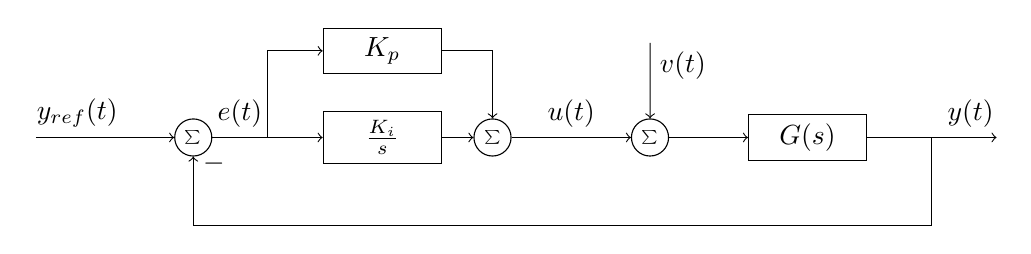
\begin{tikzpicture}[scale = 0.8, node distance=20mm, block/.style={rectangle, draw, minimum width=15mm}, sumnode/.style={circle, draw, inner sep=2pt}]

   \node[coordinate] (refinput) {};
   \node[sumnode, right of=refinput, node distance=20mm] (sumerr) {\tiny $\sum$};
   \node[block, right of=sumerr, node distance=24mm] (Ipart) {$\frac{K_i}{s}$};
   \node[block, above of=Ipart, node distance=11mm] (Ppart) {$K_p$};
   \node[sumnode, right of=Ipart, node distance=14mm] (sumcontrol) {\tiny $\sum$};
   \node[sumnode, right of=sumcontrol, node distance=20mm] (sumdist) {\tiny $\sum$};
   \node[block, right of=sumdist, node distance=20mm] (plant) {$G(s)$};
   \node[coordinate, right of=plant, node distance=24mm] (output) {};
   \node[coordinate, above of=sumdist, node distance=12mm] (dist) {};


   \draw[->] (refinput) -- node[above, pos=0.3] {$y_{ref}(t)$} (sumerr);
   \draw[->] (sumerr) -- node[above, near start] {$e(t)$} node[coordinate] (split) {} (Ipart);
   \draw[->] (split) |- (Ppart);
   \draw[->] (Ppart) -| (sumcontrol);
   \draw[->] (Ipart) -- (sumcontrol);

   \draw[->] (sumcontrol) -- node[above] {$u(t)$} (sumdist);
   \draw[->] (sumdist) -- node[above] {$$} (plant);
   \draw[->] (plant) -- node[coordinate] (measure) {} node[above, pos=0.8] {$y(t)$} (output);
   \draw[->] (measure) -- ++(0,-14mm) -| node[right, pos=0.95] {$-$} (sumerr);
   \draw[->] (dist) -- node[right, pos=0.3] {$v(t)$} (sumdist);

   \end{tikzpicture}
 \end{center}

\alert{The only way that steady-state can exist is if the input to the integrator of the controller is zero.}
\end{frame}


\section{The root locus diagram}
\label{sec:orgb6f8a9c}

\begin{frame}[label={sec:org8e0f9a4}]{Root locus}
Given loop gain \[G_o(s) = K \frac{Q(s)}{P(s)}\] how does the solutions to the characteristic equation 
\[ 1 + G_o(s) = 0 \quad \Leftrightarrow\quad P(s) + KQ(s) = 0 \]
(i.e. the \alert{poles} of the closed-loop system) depend on \(K\)?
\end{frame}

\begin{frame}[label={sec:org713aeac}]{The root locus for PI-control of the integrator}
\begin{center}
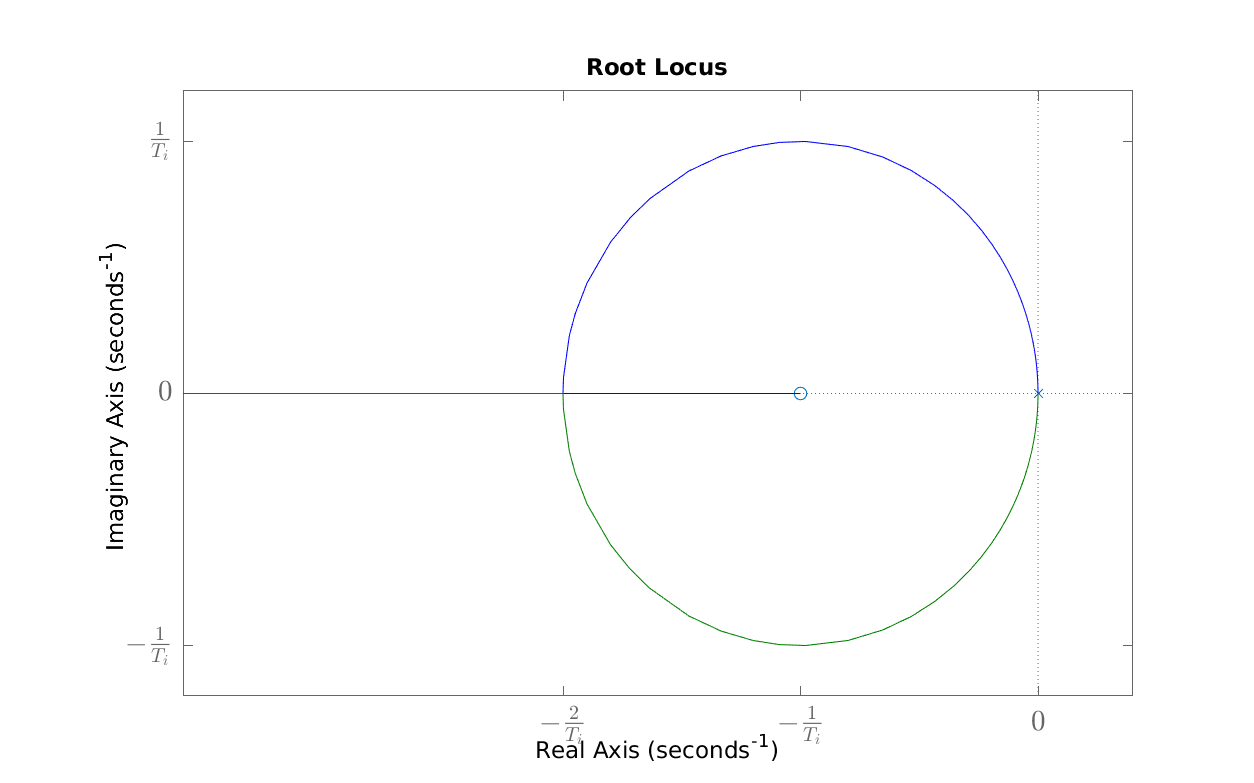
\includegraphics[width=0.8\linewidth]{../../figures/rlocus-integrator-PI}
\end{center}
\end{frame}

\begin{frame}[label={sec:org199e90e}]{Root locus question}
\end{frame}

\begin{frame}[label={sec:orgb1887b7}]{Root locus definition}
Let
\[\begin{cases} P(s)&=s^n+a_1s^{n-1}+\dots+a_n = (s-p_1)(s-p_2)\cdots(s-p_n)\\ 
Q(s)&=s^m+b_1s^{m-1}+\dots+b_m=(s-q_1)(s-q_2)\cdots(s-q_m) \end{cases},\ \ \ n\ge m \]
The root locus shows how the roots to the equation
\begin{equation}
\label{eq:P(s)+KQ(s)=0}
P(s)+K\cdot Q(s)=0,\ \ \ 0\le K<\infty
\end{equation}
depend on the parameter \(K\). The root locus consists of the set of all points in the complex plane that are roots to \eqref{eq:P(s)+KQ(s)=0} for some non-negative value of \(K\).
\end{frame}

\begin{frame}[label={sec:org2f34635}]{Characteristics of the root locus}
The polynomial \(P(s)+KQ(s)=0\) above will always have \(n\) roots. Each gives a \emph{branch} in the root locus. Since the polynomials \(P(s)\) and \(Q(s)\) have real-valued coefficients, all roots are either real or complex-conjugated pairs. This means that the root locus is \emph{symmetric about the real axis.} Other characteristics
\begin{itemize}
\item Start points - marked by crosses
\item End points - marked  by circles
\item Asymptotes
\item Pieces of the real axis
\end{itemize}
\end{frame}

\begin{frame}[label={sec:orgf80e036}]{Start- and end points}
\begin{description}
\item[{Start points}] These are the \(n\) roots of \(P(s) + KQ(s)\) for \(K=0\), i.e. the roots of \(P(s)\). These are the open-loop poles, and are marked with crosses '\(\times\)'
\item[{End points}] These are the \(m\) (finite) roots of \(P(s)+KQ(s)\) when \(K\to\infty\), and are hence the roots of \(Q(s)\). The end points are marked with circles '\(\circ\)'
\end{description}
\end{frame}

\begin{frame}[label={sec:org398a233}]{The real axis}
Those parts of the real axis that have an \alert{odd number} of real-valued start- or end points to the right (including multiplicity) belong to the root locus. 
\end{frame}


\begin{frame}[label={sec:org8aa0f2f}]{Asymptotes}
With \(n\) starting points and \(m\) end points, then \(m\) of the branches will go to end points. The rest will go out towards infinity along \(n-m\) asymptotes. The asymptotes go out symmetrically from a point on the real axis. 
\end{frame}


\begin{frame}[label={sec:org1180ef0}]{Asymptotes, directions}
The directions of the asymptotes are given by the expression
\[ \theta_k = \arg s = \frac{(2k+1)\pi}{n-m}, \; k \in \mathbb{Z} \]
Example: 6 start points and 3 end points gives \(n-m = 6-3 = 3\) and the directions

\begin{columns}
\begin{column}{0.35\columnwidth}
\[ \theta = \begin{cases} \frac{\pi}{3}, & k=0\\ \pi, & k=1\\ -\frac{\pi}{3}, & k=-1 \end{cases}. \]
\end{column}

\begin{column}{0.65\columnwidth}
\begin{center}
\includegraphics[width=0.8\linewidth]{../../MR2004/figures/root-locus-ex-3asymptotes-crop}
\end{center}
\end{column}
\end{columns}
\end{frame}

\begin{frame}[label={sec:org1d8f892}]{Asymptotes, intersection with the real axis}
\[ i.p. = \frac{ \sum_{i=0}^n p_i - \sum_{i=0}^m q_i}{n-m}, \]
where \(\{p_i\}\) are the starting points (open-loop poles) and \(\{q_i\}\) are the end points (open-loop zeros). 
\end{frame}

\section{Examples}
\label{sec:org06f35c8}
\begin{frame}[label={sec:org7a92958}]{PI-Control of the integrator}
Write the controller 
\[ F(s) = K_p + \frac{K_i}{s} = K\big(( 1 + \frac{1}{sT_i}\Big) = K/T_i \frac{sT_i + 1}{s}, \]
and let \(T_i = 2\). 
The characteristic equation can be written
\[ s^2 + \frac{K}{2}(2s + 1) = 0\]

\begin{itemize}
\item Start points: \(n=2\), in  \(s=0\)
\item End points: \(m=1\), \(s=-\frac{1}{2}\)
\item Asymptotes: \(m-n=1\), with directions \(\theta=\pi\)
\item The real line: The real-line left of the end-point is part of the root locus.
\end{itemize}
\end{frame}

\begin{frame}[label={sec:org88a3882}]{PI-Control of the integrator}
\begin{center}
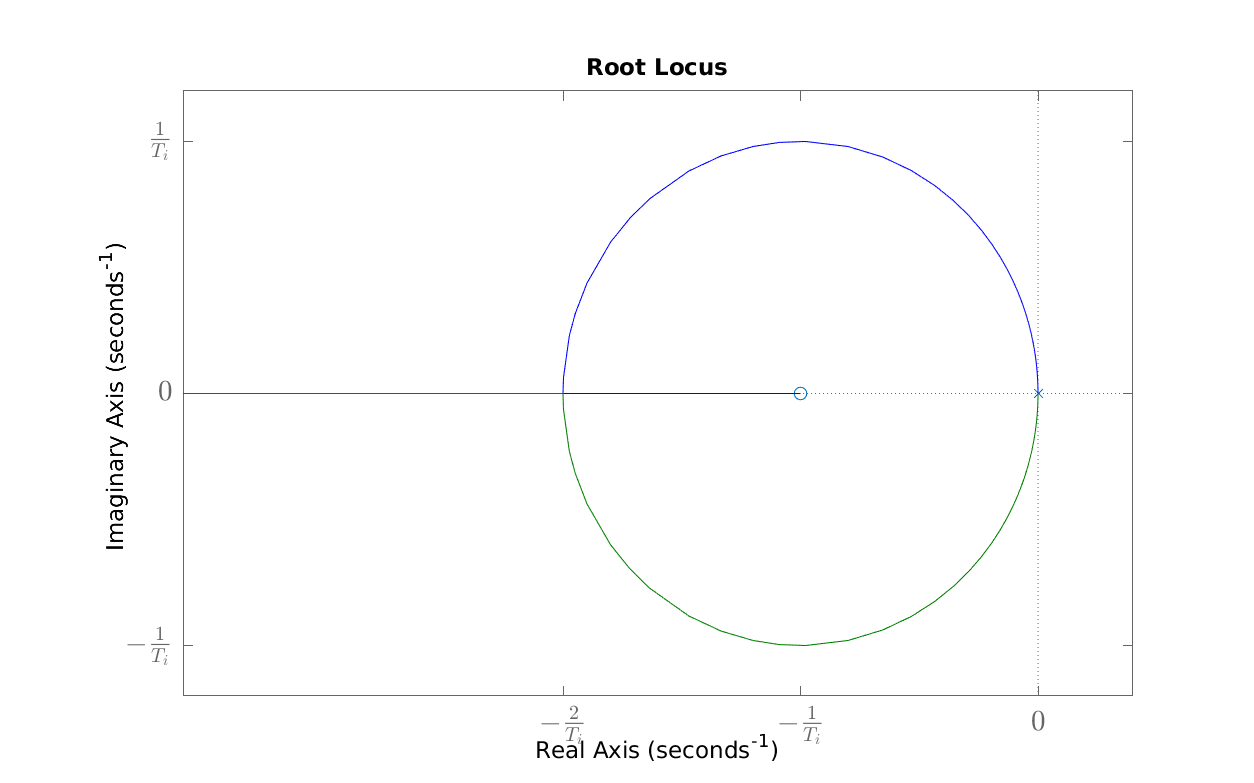
\includegraphics[width=0.8\linewidth]{../../figures/rlocus-integrator-PI}
\end{center}
\end{frame}

\begin{frame}[label={sec:org0bbe7ce}]{Do on your own: First-order system}
Instead of the plant being an integrator
\[ F(s) = \frac{1}{s}\]
consider a stable first order system
\[ F(s) = \frac{1}{s+a}\]
How does the root locus change?
\end{frame}
\end{document}